\documentclass{minimal}
\usepackage{tikz}
\usetikzlibrary{calc,trees,positioning,arrows,chains,shapes.geometric,%
	decorations.pathreplacing,decorations.pathmorphing,shapes,%
	matrix,shapes.symbols}

\tikzset{
	>=stealth',
	punktchain/.style={
		rectangle, 
		rounded corners, 
		draw=black, very thick,
		text width=10em, 
		minimum height=3em, 
		text centered, 
		on chain},
	line/.style={draw, thick, <-},
	element/.style={
		tape,
		top color=white,
		bottom color=blue!50!black!60!,
		minimum width=8em,
		draw=blue!40!black!90, very thick,
		text width=10em, 
		minimum height=3.5em, 
		text centered, 
		on chain},
	every join/.style={->, thick,shorten >=1pt},
	decoration={brace},
	tuborg/.style={decorate},
	tubnode/.style={midway, right=2pt},
}
\begin{document}
	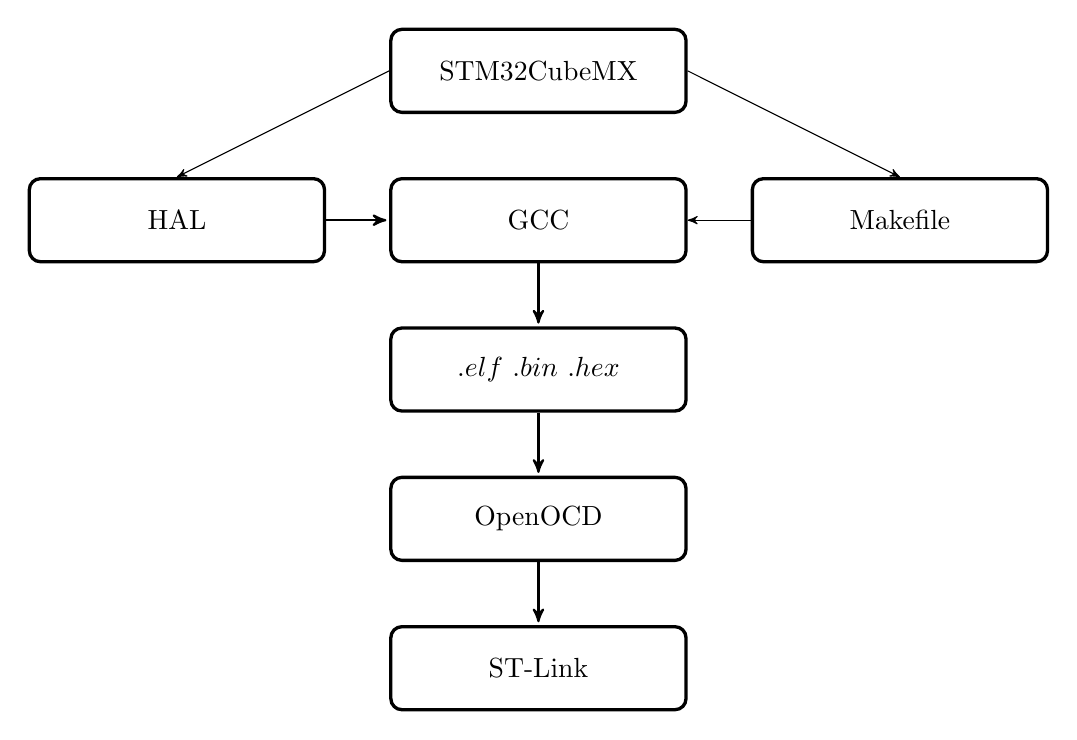
\begin{tikzpicture}
	[node distance=.8cm,
	start chain=going below,]
	
\node[punktchain, join, ] (STM) {STM32CubeMX};
\node (gcc) [punktchain ] {GCC};
\begin{scope}[start branch=top,
every join/.style={->, thick, shorten <=1pt}, ]
\node[punktchain, on chain=going left, join=by {<-}](HAL) {HAL};
\end{scope}
\begin{scope}[start branch=bottom,]
\node (makefile) [punktchain, on chain=going right] {Makefile};
\end{scope}
\node[punktchain, join,] {$.elf\ .bin\ .hex$};
\node[punktchain, join,] {OpenOCD};
\node[punktchain, join]  {ST-Link};

\draw[<-] (gcc.east) -- (makefile.west);
\draw[<-] (makefile.north) -- (STM.east);
\draw[<-] (HAL.north) -- (STM.west);
	\end{tikzpicture}
\end{document}
